\section{Concepción y Diseño}\label{section:design}

\begin{figure}
    \centering
    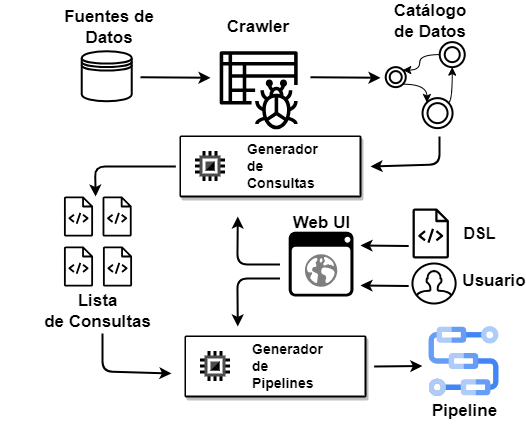
\includegraphics[width=0.60\textwidth]{Graphics/arch.drawio.png}
    \caption{Arquitectura del prototipo de AutoETL}
    \label{fig:arquitectura}
    \end{figure}

AutoETL se concibe como una herramienta para ser utilizada por los desarrolladores de almacenes de datos 
con el objetivo de aliviar la carga de trabajo en la implementaci\'on de los procesos de población de las 
estructuras analíticas. Como se observa en la Figura \ref{fig:arquitectura} los componentes de la aplicaci\'on 
est\'an dispuestos de forma secuencial para representar el flujo de trabajo de la herramienta.

\begin{itemize}
    \item El primer elemento de la arquitectura propuesta son las \textbf{Fuentes de Datos}. En esta primera concepción del 
        prototipo solo se pueden manejar bases de datos relacionales y una fuente de datos a la vez.
    \item La tarea del \textbf{Crawler} es explorar las fuentes de datos para recopilar información relevante sobre su estructura, 
        con el fin de crear el \textbf{Catálogo de Datos} a partir de dicha información.
    \item El \textbf{Catálogo de Datos} de datos es una estructura que almacena metadatos sobre las fuentes de datos, los cuales son 
        utilizados en el proceso de la generaci\'on de consultas.
    \item Los usuarios interactúan con la herramienta a través de una interfaz web. Mediante esta interfaz, especifican el modelo 
        analítico a poblar, establecen conexiones con las fuentes de datos, consultan metadatos, configuran opciones necesarias 
        para el proceso de generación de consultas y del pipeline, y finalmente ejecutan el pipeline generado. El escenario analítico 
        es especificado mediante un script del lenguaje de dominio espec\'ifico, dicho script debe ser programado por el usuario en 
        un editor de c\'odigo de su preferencia.
    \item El \textbf{Generador de Consultas} es el encargado de tomar la información proveniente del Catálogo de Datos, de la especificaci\'on
        del escenario analítico y de las configuraciones del usuario, para generar una lista de consultas que creen y pueblen el escenario 
        analítico en cuesti\'on.
    \item El \textbf{Generador de Pipelines} tiene la tarea de crear el pipeline para la población y creaci\'on del escenario analítico, partiendo 
        de la lista de consultas generadas por le generador de consultas y de las especificaciones del usuario para la creaci\'on del pipeline.
    \item Por \'ultimo, el pipeline es una estructura en la que est\'a correctamente especificado el orden de ejecuci\'on de las consultas, 
        el m\'etodo de carga y captura de los datos para la población, y la frecuencia con que se ejecutar\'a el pipeline.
\end{itemize}

En las secciones a continuación se expone de forma general el funcionamiento de
los distintos módulos del sistema y las principales consideraciones tomadas durante
su diseño.

\subsection{Crawler}

Este componente tiene la tarea de explorar las fuentes de datos para recopilar metadatos \'utiles para el proceso de generaci\'on
de consultas. Los metadatos extra\'idos son los nombres de las tablas de la base de datos fuente, por cada tabla se obtienen sus 
atributos, por cada atributo su tipo y si son llaves primarias. Adem\'as por cada tabla se obtienen los atributos que son llaves 
for\'aneas y por cada una, se extrae la tabla a la que referencian y el atributo referenciado. Con esta información se construye 
el catálogo de datos.

\subsection{Catálogo de Datos}

Una vez que los metadatos de la fuente de datos son recopilados por el Crawler se pasa a construir el Catálogo de Datos. Este componente 
es un multigrafo dirigido donde los nodos representan las tablas de la base de datos fuente y entre dos nodos $v$, $w$ 
del catálogo existe un arco $<v,w>$ por cada llave for\'anea en $v$ que referencie a un atributo de $w$. Cada nodo (tabla) guarda 
los nombres de los atributos de la tabla que representa, sus tipos y si son llaves primarias, for\'aneas o ambas. Cada arco $<v,w>$ 
guarda una tupla donde el la primera posici\'on se encuentra el nombre del atributo de $v$ que es llave for\'anea y en la segunda 
posici\'on el nombre del atributo de $w$ referenciado. N\'otese que la direcci\'on de un arco representa el sentido de la 
referencia de la llave for\'anea a la que representa.

\subsection{Lenguaje de Dominio Especifico}

Como parte de los objetivos de la presente investigaci\'on est\'a la concepción y diseño de un lenguaje de dominio 
espec\'ifico para la definici\'on de escenarios analíticos. El objetivo del lenguaje es servir de v\'inculo 
entre el modelo relacional de la fuente de datos y es modelo dimensional del escenario analítico. El lenguaje 
brinda recursos sintacticos para la especificaci\'on de tablas de dimensiones y tablas de hechos, las cuales 
en su conjunto constituyen la definicion de un esquema estrella.

La definici\'on de atributos en las tablas de hechos o de dimensi\'on constituye la base del v\'inculo entre 
el modelo relacional de la fuente y el modelo dimensional del escenario analítico. La definición de un atributo 
implica detallar la procedencia y los valores que lo constituirán, es decir, la tabla de donde se extraerán los 
valores (el 'dónde'), 
así como identificar el atributo concreto dentro de esa tabla cuyos valores se usarán para completar el atributo 
que estamos definiendo (el 'con qué'). Este proceso garantiza que cada atributo se defina de manera clara y que 
se alimente correctamente con los datos pertinentes. De esta forma se entrelazan la definici\'on relacional 
de la fuente de datos con el modelo dimensional del esquema estrella. A continuación se presenta la gramática 
libre del contexto que da definición al DSL propuesto. Las palabras en may\'uscula indican no terminales y 
las palabras en min\'uscula indican terminales.

\begin{lstlisting}[caption={Gram\'atica libre del contexto del lenguaje de dominio espec\'ifico}]
    S' -> Dimensional_Model
    Dimensional_Model -> List_Dimensional_Tables
    List_Dimensional_Tables -> Dimensional_Table
                    | List_Dimensional_Tables Dimensional_Table

    Dimensional_Table -> dimension ID { List_Attr_Def }
                       | fact ID { List_Attr_Def }

    List_Attr_Def -> Attr_Def
                   | List_Attr_Def Attr_Def

    Attr_Def -> Attr_Expression Type Alias

    Attr_Expression -> T X
    X -> + T X | - T X | empty
    T -> F Y
    Y -> * F Y | / F Y | empty
    F -> Attr | number | (Attr_Expression)

    Attr -> Table : ID Modifier
          | Table : Func ( ID )
          | Table : sum ( ID )
          | Table : avg ( ID )
          | Table : count ( ID )
          | Table : max ( ID )
          | Table : min ( ID )

    Table -> ID | self

    Func -> weekday | monthstr

    Alias -> as ID | empty

    Type -> int | str | date | datetime | serial | float | numeric 
          | empty

    Modifier -> pk | fk to ID . ID | empty
\end{lstlisting}

%TODO: Agregar definicion de multigrafo en el marco teorico

Tal y como dicta la gramática, un modelo dimensional (Dimensional\_Model), 
en el contexto del DSL, est\'a compuesto por una lista de tablas 
dimensionales (List\_Dimensional\_Tables). 

Una lista de tablas dimensionales est\'a compuesta por al menos una definici\'on de tabla dimensional 
(Dimensional\_Table), aunque es cierto que un esquema estrella no tiene sentido si tiene una sola tabla 
de dimensi\'on o una sola tabla de hechos, expresar la restricci\'on en la gramática de que una lista de 
tablas dimensionales debe tener al menos una tabla de dimensi\'on y una tabla de hechos es un proceso 
engorroso que puede atentar contra la legibilidad de la gramática, por tanto se decide dejar dicha 
comprobaci\'on para los chequeos sem\'anticos que se le efect\'uan a las instancias del lenguaje provistas 
por el usuario, luego de ser parseadas. 

Luego, la 
definición de una tabla dimensional (Dimensional\_Table) consta de la palabra clave dimension o fact, 
en caso de querer definir una dimension o una tabla de hechos respectivamente, un nombre para dicha tabla 
(ID), llaves con funci\'on delimitadora ({}) y dentro de estas una lista de definiciones de atributos
(List\_Attr\_Def). 

Una lista de definiciones de atributos est\'a compuesta por al menos una definición de atributo (Attr\_Def). 
La definición de un atributo consta de una expresión de atributos (Attr\_Expression), un tipo para el atributo 
definido, dicho tipo puede especificarse o no, y un alias que en caso de no ser vacío ser\'a el nombre del 
atributo en el esquema estrella. Una expresión de atributos (Attr\_Expression) no es m\'as que 
un recurso gramatical para expresar que una definición de atributo puede ser tanto un solo atributo (Attr)
como una expresi\'on aritm\'etica en la que pueden participar atributos y n\'umeros. 

Un atributo (Attr) es la representaci\'on en el DSL de un atributo de la fuente de datos. Est\'a compuesto, 
fundamentalmente, 
por el nombre de la tabla de la fuente de datos (Table), dos puntos y el nombre del atributo de dicha tabla 
de donde se obtendr\'an los valores (ID). Adem\'as puede contener especificaciones de modificadores (Modifier), 
los cuales pueden ser especificaciones de llave primaria o llave for\'anea. En esta primera versi\'on del 
DSL un atributo puede ser llave primaria o llave for\'anea, pero no los dos a la vez. Tambi\'en, a los valores
extra\'idos del atributo con nombre (ID) y tabla (Table) se le puede aplicar funciones o agregaciones. Las 
funciones de agregaci\'on implementadas son suma (sum), promedio (avg), conteo (count), m\'aximo (max) y 
m\'inimo (min). Las funciones implementadas en esta primera versi\'on son weekday, la cual a partir de 
una fecha devuelve el d\'ia de la semana, y monthstr que devuelve el nombre del mes de una fecha pasada 
como argumento. La palabra reservada self solo se debe usar para declarar la tabla en la definición de atributos 
que sean llaves primarias autogeneradas para las tablas de hechos.

Los tipos manejados por el lenguaje son gen\'ericos y facilmente mapeables con los tipos de los sistemas de 
gesti\'on de bases de datos relacionales m\'as usados. El tipo int engloba a los n\'umeros enteros. 
Al tipo str pertenecen las cadenas de texto. Los tipos date y datetime agrupan a las fechas y a las fechas con 
hora respectivamente. El tipo serial se usa para las llaves primarias autogeneradas. El tipo float 
representa a los n\'umeros con coma flotante. Finalmente, al tipo numeric pertenecen todos los valores numéricos.

En caso de que una definición de un atributo solo contenga un atributo de una tabla de la fuente no es necesario 
especificar el tipo, pues el sistema autom\'aticamente asignar\'a el tipo del atributo fuente al tipo del 
atributo que est\'a siendo definido. Sin embargo si se define un atributo compuesto, es decir, un atributo que 
en su definición participe m\'as de un atributo de la fuente, es necesario especificar el tipo pues el sistema 
no es capaz de inferirlo.

Para especificar una llave for\'anea se deben escribir las palabras reservadas fk y to y luego especificar 
el nombre de una tabla del esquema estrella, un punto y el atributo referenciado. 